\chapter{Knowledge And Conflict In Relationship}

This chapter follows J. Krishnamurti's second San Diego conversation with Dr. Alan W. Anderson on knowledge and conflict in human relationship. The source is not a blackboard lecture with equations; there are no validated screenshots of written mathematics or diagrams. Still, the dialogue has a precise logical structure. We will make that structure visible with a small amount of editorial notation, always keeping the spoken inquiry primary: thought, image, knowledge, observer, division, relationship, freedom, attention, and transformation.

\section{The Observer As The Past}

Anderson begins by recalling the previous conversation. They had distinguished the fact that ``the world is me and I am the world'' from the confusion of taking the description for the described. That distinction now presses toward a new question: what is the observer who makes this mistake, and can that observer relate to what is observed in a different way?

Krishnamurti's reply is immediate. The observer is not an independent inner witness standing outside confusion. The observer is the past. It is made of thought, and thought is made of accumulated knowledge, experience, memory, hurt, hope, image, tradition, and conditioning. In compact editorial notation, we can write the first movement of the conversation as
\begin{equation}
\mathrm{Thought}=\mathrm{Past}.
\end{equation}
This does not mean that Krishnamurti offered an algebra of consciousness. It is only a faithful shorthand for the spoken claim that thought is the response of the past.

The next step is just as important:
\begin{equation}
\mathrm{Observer}=\mathrm{Past}.
\end{equation}
The observer, when he observes, looks from the background of what has been. He looks with memories, experiences, knowledge, hurts, despairs, hopes. Therefore the observer is already carrying a division into the act of observation.

\begin{definition}
In this chapter, \(O\) denotes the observer as Krishnamurti describes it: not a pure faculty of awareness, but the past operating as thought, knowledge, memory, image, and conditioned response.
\end{definition}

With that notation the initial diagnosis can be compressed as
\begin{equation}
O=\mathrm{Past}=\mathrm{Knowledge}+\mathrm{Experience}+\mathrm{Memory}+\mathrm{Image}.
\end{equation}
The plus signs here do not indicate a literal sum. They mark the main components named in the dialogue. The point is that the observer is not free from the known; the observer is the known.

\begin{proposition}
Where observation is governed by \(O\), observation is already divided.
\end{proposition}

\begin{proof}
Krishnamurti identifies \(O\) with the past. The past includes memory, image, hurt, tradition, and conditioned response. When \(O\) observes, it therefore observes through these residues. Such observation is not whole; it separates the observer from the observed. Thus observation governed by \(O\) is already divided.
\end{proof}

The phrase ``I'' is then drawn into the same structure. The ``I'' that speaks from this background is not separate from the observer; it is the observer. Hence the chapter's working notation may also record:
\begin{equation}
\mathrm{I}=O=\mathrm{Past}.
\end{equation}
This is the first severe correction in the conversation. The problem is not merely that the observer uses knowledge wrongly. The observer is the accumulated field of the known.

\section{Freedom From The Known And Creative Action}

Once the observer has been identified with the past, the next question arises naturally: can the mind be free from the known? Krishnamurti does not pose this as an abstract ideal. If the known is only the repetition of the past, then action born from the known will also be repetition, however modified.

The dialogue then turns to the word ``creative.'' Krishnamurti is careful to separate creative action from what people commonly call creativity: creative writing, creative pictures, creative this and that. In that ordinary use, the new may be merely novel. It may attract attention, appear eccentric, or succeed in surprising others, while still belonging to the same structure of repetition.

We may record the distinction as
\begin{align}
\mathrm{Novelty} &= \mathrm{Modified\ Repetition},\\
\mathrm{Creative\ Action} &\neq \mathrm{Novelty}.
\end{align}
The difference is not cosmetic. Novelty is still tied to the past. Creative action, in the deeper sense intended here, requires something totally new being born.

\subsection{Question \& Answer}

\paragraph{Question.}
Does freedom from the known mean rejecting knowledge?

\paragraph{Answer.}
No. Krishnamurti explicitly says that freedom is not the negation of the known. Freedom comes through understanding the known. The known must be understood in its actual operation: where it functions properly, and where it becomes image, barrier, and division.

The local structure is therefore:
\begin{equation}
\mathrm{Freedom\ from\ the\ Known}
\neq
\mathrm{Negation\ of\ Knowledge}.
\end{equation}
More carefully:
\begin{equation}
\mathrm{Understanding\ of\ the\ Known}
\longrightarrow
\mathrm{Intelligence}
\longrightarrow
\mathrm{Freedom}.
\end{equation}

This point prevents a common misunderstanding. The chapter must not make Krishnamurti sound as though he is recommending ignorance or rejecting practical knowledge. He is asking whether the mind can understand the known so completely that it is no longer bound by it in relationship.

\begin{figure}
\centering
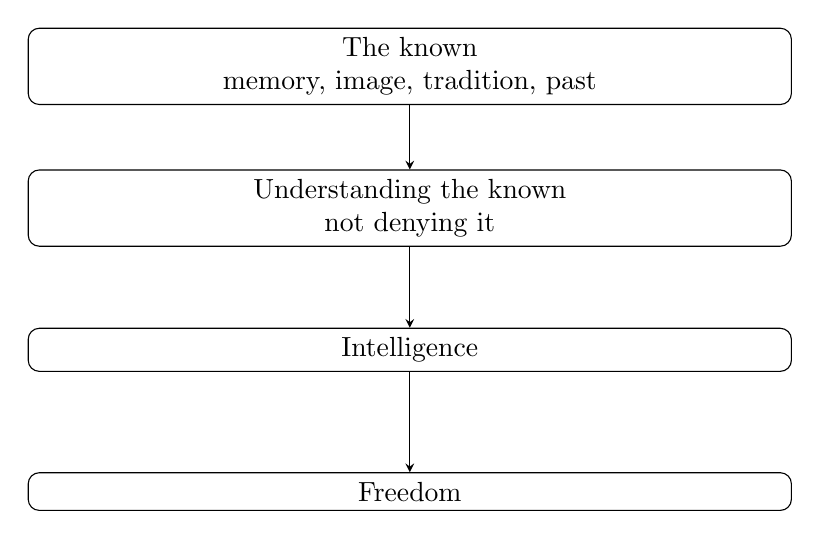
\begin{tikzpicture}[>=stealth]
\node[draw, rounded corners, align=center, text width=0.78\linewidth] (known) at (0,0) {The known\\memory, image, tradition, past};
\node[draw, rounded corners, align=center, text width=0.78\linewidth] (understand) at (0,-1.8) {Understanding the known\\not denying it};
\node[draw, rounded corners, align=center, text width=0.78\linewidth] (intelligence) at (0,-3.6) {Intelligence};
\node[draw, rounded corners, align=center, text width=0.78\linewidth] (freedom) at (0,-5.4) {Freedom};
\draw[->] (known) -- (understand);
\draw[->] (understand) -- (intelligence);
\draw[->] (intelligence) -- (freedom);
\end{tikzpicture}
\caption{A transcript-derived reconstruction of the movement from understanding the known to freedom.}
\end{figure}

\section{Knowledge As Function, Knowledge As Division}

The conversation next makes a crucial turn. Knowledge is necessary. We need knowledge to go home, to speak English, to write a letter, to function in ordinary mechanical ways. Krishnamurti is not erasing the practical order of life.

Let \(K_f\) denote functional knowledge and \(K_r\) denote knowledge operating in relationship as image, memory, tradition, and observer. Then the lecture's distinction is:
\begin{equation}
K_f \neq K_r.
\end{equation}
Functional knowledge is practical and necessary. Relational knowledge, when it is the accumulated image of another person, becomes separative.

\begin{table}
\centering
\begin{tabular}{p{0.42\linewidth} p{0.42\linewidth}}
\hline
\(K_f\): functional knowledge & \(K_r\): knowledge in relationship \\
\hline
Going home & Image of another person \\
Speaking a language & Memory of hurt or demand \\
Writing a letter & Tradition and conditioning \\
Mechanical operation & Observer acting as the past \\
Necessary for function & Barrier between you and me \\
\hline
\end{tabular}
\caption{The dialogue's central distinction between functional knowledge and knowledge as image in relationship.}
\end{table}

The transition is exact. Krishnamurti says, in effect: knowledge is necessary to act in a practical sense; now see what happens if that knowledge is used in relationship with another human being. It brings about a barrier, a division between you and me.

We can write the working chain as
\begin{equation}
K_r \longrightarrow \mathrm{Barrier}
\longrightarrow \mathrm{Division}
\longrightarrow \mathrm{Conflict}.
\end{equation}
This is the chapter's first explicit derivation of conflict. It does not begin with society, nation, or ideology. It begins with the observer as the past entering relationship.

\begin{proposition}
Knowledge as image in relationship produces conflict.
\end{proposition}

\begin{proof}
In the dialogue, knowledge in relationship means tradition, memory, past experience, and image. Such knowledge stands between two people as a barrier. A barrier creates division. Krishnamurti repeatedly states that where there is division there must be conflict. Hence knowledge as image in relationship produces conflict.
\end{proof}

The same pattern then scales outward. Division between husband and wife, between one person and another, between India and Pakistan, America and Russia, one religion and another: the form changes, but the structure remains the same.

\section{Relationship And The Place Of The Observer}

The lecture now reaches its central question: what place has knowledge in human relationship? More sharply: what place has the observer in human relationship?

Krishnamurti insists that relationship is not peripheral. There is no life without relationship. Even the person who retires into a monastery remains related: to the past, to a savior, to a rule, to an image, to a tradition. Relationship is the field in which the whole problem is tested.

The question must be preserved in its repeated form because the repetition is part of the inquiry:
\begin{equation}
\text{What place has } O \text{ in relationship?}
\end{equation}
At first, one might answer that the observer has a place as the one who must learn how to relate. But Krishnamurti's answer moves in the opposite direction. The observer is the factor of division. If the observer enters relationship, the relationship is no longer actual relationship.

\subsection{Question \& Answer}

\paragraph{Question.}
Has the observer any place in human relationship?

\paragraph{Answer.}
Krishnamurti's answer is no. The moment the observer comes into relationship, division has entered. And where there is division, relationship is already broken. What appears to be relationship may be habit, dependence, sexual contact, social arrangement, or mutual use, but the actual relationship is absent.

In compact notation:
\begin{align}
O \in \mathrm{Relationship}
&\longrightarrow \mathrm{Division},\\
\mathrm{Division}
&\longrightarrow \mathrm{No\ Actual\ Relationship}.
\end{align}

This is why the theoretical statement ``the world is me and I am the world'' is not enough. If the mind turns that statement into an idea, a concept, or a formula to live by, it has again abstracted from reality. The idea becomes another piece of knowledge in the destructive sense. The observer has simply appropriated the statement and continued.

\begin{figure}
\centering
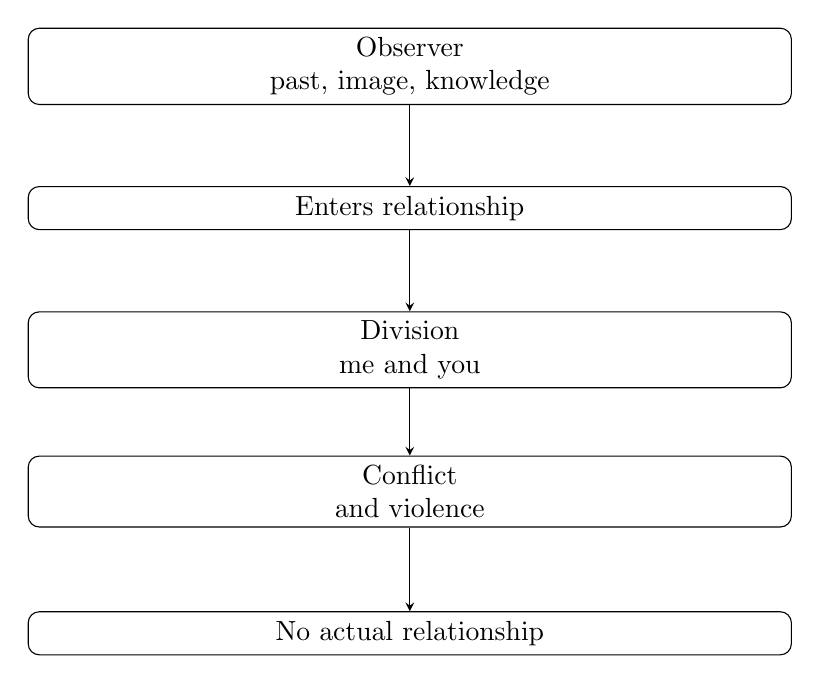
\begin{tikzpicture}[>=stealth]
\node[draw, rounded corners, align=center, text width=0.78\linewidth] (observer) at (0,0) {Observer\\past, image, knowledge};
\node[draw, rounded corners, align=center, text width=0.78\linewidth] (relationship) at (0,-1.8) {Enters relationship};
\node[draw, rounded corners, align=center, text width=0.78\linewidth] (division) at (0,-3.6) {Division\\me and you};
\node[draw, rounded corners, align=center, text width=0.78\linewidth] (conflict) at (0,-5.4) {Conflict\\and violence};
\node[draw, rounded corners, align=center, text width=0.78\linewidth] (absence) at (0,-7.2) {No actual relationship};
\draw[->] (observer) -- (relationship);
\draw[->] (relationship) -- (division);
\draw[->] (division) -- (conflict);
\draw[->] (conflict) -- (absence);
\end{tikzpicture}
\caption{The observer as the factor of division in relationship.}
\end{figure}

The everyday examples matter. One may call another person husband, wife, brother, friend. Yet if each is pursuing private ambition, private success, private hurt, private demand, then the name of relationship conceals separation. The observer, as the past, is the point at which relationship fails.

\section{Freedom, Austerity, Order, And Virtue}

Having established the problem of knowledge in relationship, the dialogue turns toward freedom. Freedom is not a vague condition and not an escape from practical life. Krishnamurti links it with attention, austerity, order, virtue, and action.

He speaks of religion as gathering energy to be attentive. The etymological claim should not be overburdened, but the movement in the dialogue is clear: attention is not casual looking. It gathers the whole energy of the mind. Freedom, in this context, means a total negation of the observer.

The word austerity enters next. Anderson and Krishnamurti distinguish the dry, brittle sense of austerity from the inward austerity that belongs to freedom. Austerity does not produce freedom as a method. Rather, the austerity being discussed belongs to freedom from the observer.

The practical question then becomes:
\begin{equation}
\text{Can a human being live in relationship, in freedom, and operate in } K_f?
\end{equation}
This is one of the most important balancing statements in the dialogue. The point is not to abolish knowledge. It is to live in freedom and yet operate in the field of knowledge where knowledge has its proper function.

Freedom is then tied to order:
\begin{equation}
\mathrm{Freedom} \longrightarrow \mathrm{Order}.
\end{equation}
And Krishnamurti adds:
\begin{equation}
\mathrm{Order}=\mathrm{Virtue}.
\end{equation}
Anderson helps recover the step: virtue is not a moral decoration but the ability to act. If action is merely reaction, it is repetition. Thus:
\begin{align}
\mathrm{Reaction} &= \mathrm{Repetition},\\
\mathrm{Action} &\neq \mathrm{Reaction}.
\end{align}
Here action means creative action in the earlier sense: not modified past, not novelty, not eccentricity, but something that is not born from the observer.

\section{The Fragment Cannot Become The Whole}

The conversation now names a difficult obstacle. Anderson observes that the reference for Krishnamurti's question is always a totality, while the condition from which the question is usually heard is fragmentary. The fragment wants to move toward the whole, but Krishnamurti agrees: there is no such passage.

We can state the point as a proposition:
\begin{proposition}
The fragment cannot become the whole by a movement of the fragment.
\end{proposition}

\begin{proof}
The fragment is already part of the divided structure. Any movement it makes from its own center remains a movement of division. If the fragment tries to become the whole, the attempt is still governed by the fragment. Therefore the passage from fragment to whole cannot be produced by the fragment itself.
\end{proof}

The notation is stark:
\begin{equation}
\mathrm{Fragment} \nrightarrow \mathrm{Whole}.
\end{equation}
This should not be read as despair. It is a warning against gradualism inside disorder. If the observer is the past, and the observer tries to construct freedom as an ideal, then the construction is still the past. If disorder modifies itself, the result is still disorder.

That final claim can be written:
\begin{equation}
\mathrm{Modification\ of\ Disorder}
=
\mathrm{More\ of\ the\ Same}.
\end{equation}

\subsection{Question \& Answer}

\paragraph{Question.}
Can disorder gradually become order?

\paragraph{Answer.}
Not in the sense the dialogue is examining. The fragment, acting as fragment, cannot become the whole. The observer, acting as observer, cannot produce freedom from the observer. Any progress made inside disorder remains a proliferation of the same structure unless there is a different kind of observation.

\begin{figure}
\centering
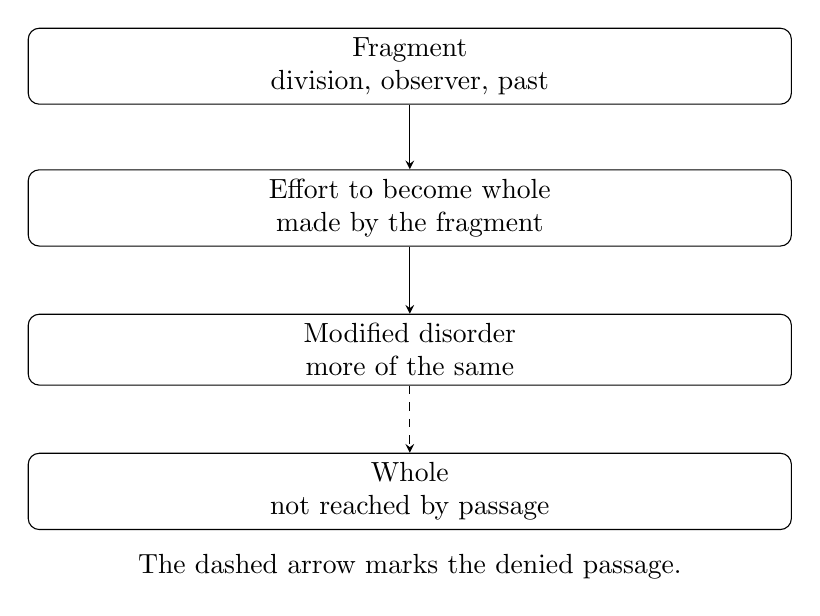
\begin{tikzpicture}[>=stealth]
\node[draw, rounded corners, align=center, text width=0.78\linewidth] (fragment) at (0,0) {Fragment\\division, observer, past};
\node[draw, rounded corners, align=center, text width=0.78\linewidth] (effort) at (0,-1.8) {Effort to become whole\\made by the fragment};
\node[draw, rounded corners, align=center, text width=0.78\linewidth] (more) at (0,-3.6) {Modified disorder\\more of the same};
\node[draw, rounded corners, align=center, text width=0.78\linewidth] (whole) at (0,-5.4) {Whole\\not reached by passage};
\draw[->] (fragment) -- (effort);
\draw[->] (effort) -- (more);
\draw[->, dashed] (more) -- (whole);
\node[align=center, text width=0.72\linewidth] at (0,-6.35) {The dashed arrow marks the denied passage.};
\end{tikzpicture}
\caption{A reconstruction of the dialogue's claim that the fragment cannot become the whole through gradual movement.}
\end{figure}

\section{Listening, Regeneration, And The Urgency Of Relationship}

The final movement of the dialogue asks whether a mind that has evolved in separation, contradiction, duality, and fragmentation can undergo regeneration. Krishnamurti is careful: this regeneration is not produced by influence, propaganda, threat, punishment, or reward. If change comes because one seeks reward, it has not changed.

The issue returns to observation:
\begin{equation}
\mathrm{Observation\ by\ } O \longrightarrow \mathrm{Conflict}.
\end{equation}
But the dialogue also points to another possibility:
\begin{equation}
\mathrm{Observation\ without\ } O
\longrightarrow
\mathrm{Regeneration}.
\end{equation}
This is a cautious reconstruction of the spoken movement, not a method. Krishnamurti does not give steps, exercises, or a program. He asks whether the fact of division can be observed without the observer. Only then, he says, is there regeneration.

Anderson hears the severity of the point. If disorder persists, it cannot change itself. Any modification is more of the same. Krishnamurti then turns to listening. The difficulty is not that the argument is verbally obscure; the difficulty is that most people do not listen. If they listen at all, they listen through conclusions.

Listening therefore becomes more than reception of words. It is the act in which the observer may be absent. The dialogue says, in effect:
\begin{equation}
\mathrm{Listening\ through\ Conclusions}
\longrightarrow
\mathrm{Continuation\ of\ the\ Known}.
\end{equation}
By contrast:
\begin{equation}
\mathrm{Listening\ itself}
\longrightarrow
\mathrm{Attention}.
\end{equation}

The examples at the end are deliberately concrete: academic conferences where nobody listens, ordinary social babble, the burning house, the urgency of relationship. The point is not rhetorical. If the house is burning, we do not first debate the biography of the person who lit the fire. We act. Relationship, for Krishnamurti, is the burning house. If relationship contains conflict, society will extend that conflict through education, sovereignty, ideology, and all the arrangements of collective life.

The closing triad is therefore:
\begin{equation}
\mathrm{Relationship}+\mathrm{Freedom}+\mathrm{Knowledge}.
\end{equation}
These are not three detachable subjects. The serious human being must give total attention to their relation.

\section{Summary}

The conversation begins with the observer and ends with attention. Its central discovery is that the observer is not outside the disorder it observes. The observer is the past: thought, memory, knowledge, image, hurt, hope, and conditioning. When such an observer enters relationship, it divides; where there is division, there is conflict; where conflict becomes the basis of life, society reproduces violence.

The chapter's compact structure is:
\begin{align}
\mathrm{Thought} &= \mathrm{Past},\\
O &= \mathrm{Past},\\
O &\longrightarrow \mathrm{Division},\\
\mathrm{Division} &\longrightarrow \mathrm{Conflict},\\
K_r &\longrightarrow \mathrm{No\ Actual\ Relationship}.
\end{align}
Against this, Krishnamurti does not offer rejection of knowledge. He distinguishes functional knowledge from knowledge as image in relationship. Knowledge is necessary for function, but when it becomes the observer between human beings, it destroys relationship.

The possibility opened by the dialogue is austere and exact: freedom is not disorder, and it is not gradual improvement of the fragment. Freedom is order, order is virtue, and virtue is living action rather than repetition. The question left for the continuing inquiry is whether there can be observation without the observer, and whether in such attention there is the beginning of regeneration.